\chapter{Metodologia}

Este capítulo apresenta a metodologia adotada no desenvolvimento e na validação da aplicação web proposta para o planejamento de redes ópticas \gls{pon}. Inicialmente, são descritas a natureza da pesquisa e a abordagem metodológica do estudo. Em seguida, detalham-se a arquitetura da solução, as tecnologias empregadas, o processo de desenvolvimento do sistema e os procedimentos definidos para sua validação e análise dos resultados.

\section{Caracterização da Pesquisa}

Esta pesquisa caracteriza-se como aplicada, pois busca desenvolver uma solução computacional voltada à resolução de um problema prático no contexto do planejamento de redes ópticas \gls{ftth} baseadas em \gls{pon}. Quanto aos procedimentos, apresenta natureza experimental, uma vez que envolve a implementação de uma aplicação web interativa e sua avaliação em cenários controlados. Em relação aos objetivos, possui caráter exploratório e descritivo, pois investiga de que modo a integração entre modelagem visual da topologia, cálculo automatizado do orçamento óptico e armazenamento estruturado das informações do projeto pode contribuir para tornar o processo de planejamento mais claro, ágil e confiável \cite{gil2008metodos,prodanov2013metodologia}.

Quanto à abordagem metodológica, o estudo adota método misto, com predominância qualitativa e apoio quantitativo. A dimensão qualitativa está associada à análise da adequação da arquitetura proposta, da interface interativa e do fluxo de uso da ferramenta no contexto do planejamento técnico de redes ópticas. Já a dimensão quantitativa concentra-se na etapa de validação, por meio da comparação entre os valores calculados pelo sistema e os resultados esperados para cenários de teste previamente definidos, além da observação de indicadores de consistência funcional e desempenho. Desse modo, o trabalho envolve tanto o desenvolvimento do software quanto a análise de seu comportamento e de sua capacidade de atender aos objetivos técnicos estabelecidos \cite{creswell2014research}.

Em conformidade com as orientações do \gls{mec} e do \gls{cnpq} sobre integridade científica, declara-se o uso de ferramentas de \gls{ia} generativa durante a elaboração deste trabalho. O Microsoft Copilot foi utilizado como apoio à pesquisa bibliográfica, auxiliando na busca de artigos, livros e referências, bem como na revisão textual. As ferramentas Gemini e ChatGPT foram empregadas na elaboração de imagens e diagramas técnicos, enquanto o Grammarly foi utilizado na verificação ortográfica e gramatical do texto. Ressalta-se, contudo, que a responsabilidade pelo conteúdo intelectual do trabalho, pela seleção e validação das referências, pela veracidade dos dados técnicos sobre redes ópticas, pela análise crítica dos resultados e pela redação final permanece integralmente sob a autoria do pesquisador, assegurando a originalidade e a rastreabilidade do processo científico.

\section{Arquitetura da Solução}

O sistema proposto é estruturado segundo uma arquitetura cliente-servidor. Nessa configuração, o \textit{frontend} concentra a interação com o usuário e a representação gráfica da rede \gls{pon}, enquanto o \textit{backend} reúne a lógica de negócio, as validações e a disponibilização dos dados. Essa divisão favorece a separação de responsabilidades, a modularidade do sistema e a evolução independente entre interface e processamento.

A estrutura da aplicação pode ser compreendida a partir de três partes principais. A primeira corresponde à apresentação, implementada em ambiente web, na qual o usuário constrói visualmente a topologia da rede e acompanha os resultados após o recálculo automático provocado por alterações. A segunda refere-se ao processamento, responsável por tratar as operações solicitadas, validar os parâmetros informados e executar as rotinas de cálculo do orçamento óptico com base nos elementos modelados. A terceira diz respeito aos dados, destinados ao armazenamento estruturado das informações do projeto, incluindo topologia, parâmetros técnicos e resultados calculados. Essa arquitetura será complementada por diagramas e fluxos de interação, de modo a explicitar a comunicação entre as partes do sistema e facilitar a compreensão de seu funcionamento.

Na Figura~\ref{fig:arquitetura_solucao}, observa-se a estrutura da aplicação e o fluxo de comunicação entre seus principais elementos. O diagrama evidencia a interação entre a interface web, responsável pela modelagem visual, o módulo de processamento, no qual são executadas as rotinas de cálculo e verificação, e a camada de dados, destinada ao armazenamento estruturado das informações do projeto.

\begin{figure}[htb]
	\caption{Arquitetura da solução proposta}
	\label{fig:arquitetura_solucao}
    \centering
    \parbox{16cm}{
		\centering
		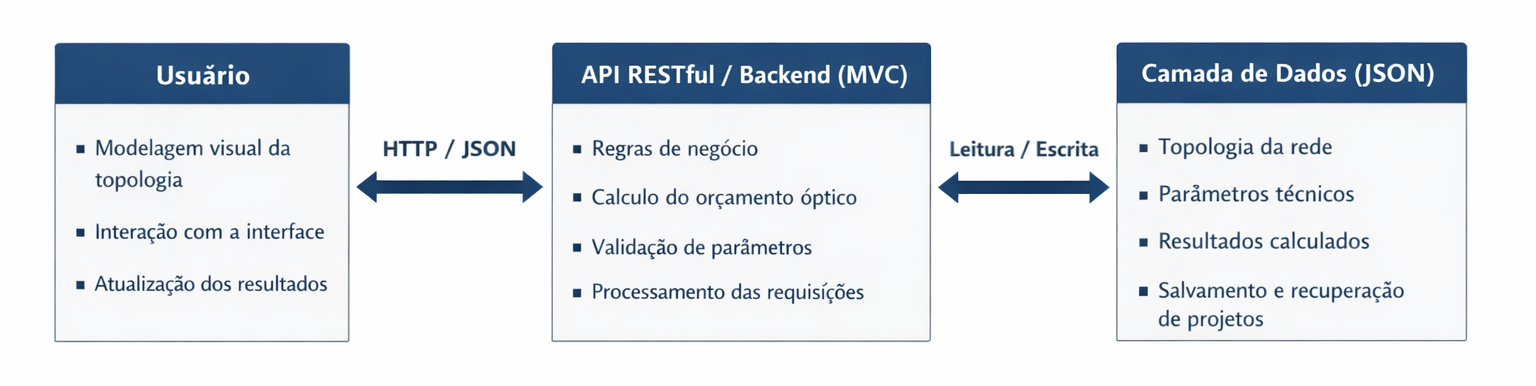
\includegraphics[width=\textwidth]{images/arquitetura_solucao.png}
		\par\footnotesize Fonte: Elaboração própria com auxilio de IA.
    }
\end{figure}

\section{Ferramentas e Tecnologias}

O desenvolvimento da aplicação será baseado em tecnologias voltadas a sistemas web interativos e modulares. No \textit{frontend}, serão utilizados \gls{html}, \gls{css} e \textit{JavaScript}, com apoio da biblioteca D3.js para a visualização interativa da topologia da rede \gls{pon}. No \textit{backend}, será empregada a linguagem Python, devido à sua simplicidade e adequação à implementação da lógica de negócio e dos cálculos de orçamento óptico. A \gls{api} \textit{RESTful} será desenvolvida com FastAPI, responsável pelo processamento das requisições, validação de dados e organização dos serviços conforme o padrão \gls{mvc}. A comunicação entre os componentes ocorrerá via \gls{http}, utilizando o formato \gls{json} para a troca de dados.

O ambiente de execução será padronizado com o uso de contêineres \textit{Docker}, garantindo a portabilidade da aplicação. Os projetos serão armazenados em arquivos no formato \gls{json}, permitindo a persistência, a recuperação e a reutilização das topologias desenvolvidas. Ferramentas de versionamento e apoio ao desenvolvimento serão empregadas ao longo da implementação, incluindo o uso da plataforma GitHub para gerenciamento e versionamento do código-fonte, bem como o ambiente de desenvolvimento Visual Studio Code (VS Code) para suporte à codificação, depuração e organização da aplicação.

\section{Metodologia de Desenvolvimento}

O desenvolvimento seguirá uma abordagem incremental e iterativa, permitindo a evolução progressiva do sistema a partir de versões parciais. Inicialmente, serão realizados o levantamento e a consolidação dos requisitos, considerando o objetivo geral do trabalho e os objetivos específicos relacionados à modelagem visual da topologia, ao cálculo automático do orçamento óptico, à definição da arquitetura de software e à persistência dos projetos. Em seguida, será conduzido o planejamento arquitetural, com definição das responsabilidades dos principais módulos e dos fluxos de comunicação necessários ao funcionamento da aplicação. O fluxo geral desse processo é sintetizado na Figura~\ref{fig:fluxo_metodologia_desenvolvimento}, que organiza as etapas adotadas neste trabalho \cite{pressman2014software,sommerville2016software}.

\begin{figure}[htb]
	\caption{Fluxo da metodologia de desenvolvimento}
	\label{fig:fluxo_metodologia_desenvolvimento}
    \centering
    \parbox{16cm}{
		\centering
		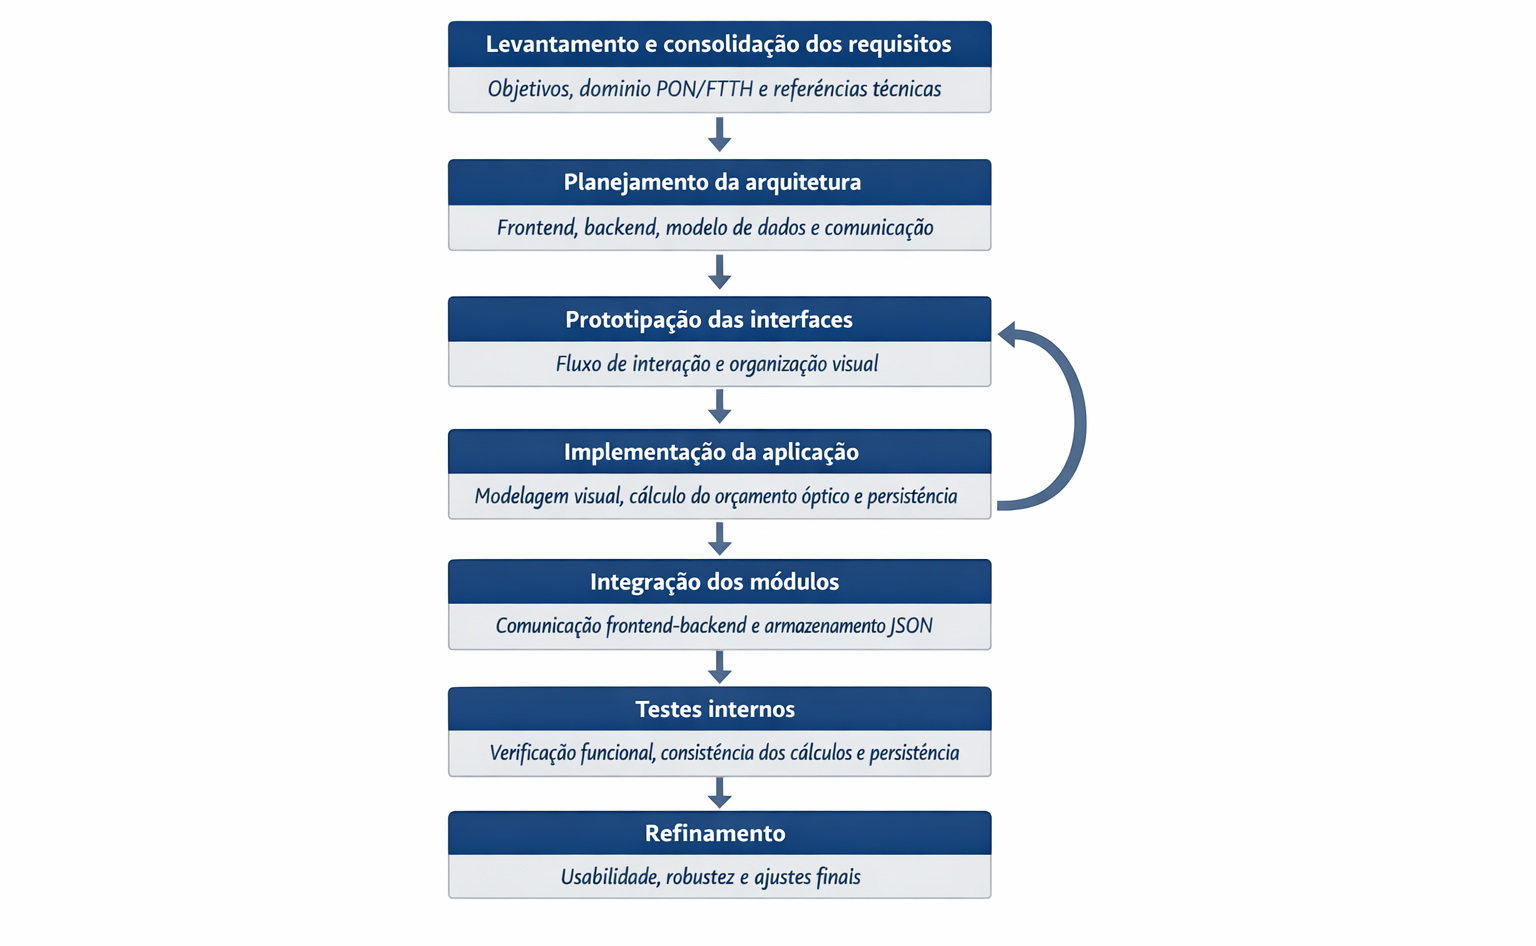
\includegraphics[width=\textwidth]{images/fluxo_metodologia_desenvolvimento.png}
		\par\footnotesize Fonte: Elaboração própria com auxilio de IA.
    }
\end{figure}

A Figura~\ref{fig:fluxo_metodologia_desenvolvimento}, demonstra as etapas de levantamento de requisitos, planejamento da arquitetura, prototipação das interfaces, implementação, integração dos módulos, testes internos e refinamento. A presença de realimentação entre as etapas finais evidencia o caráter iterativo do processo, no qual os resultados obtidos nos testes orientam ajustes sucessivos no sistema.

Na sequência, serão executadas as etapas de prototipação das interfaces, implementação da visualização para construção da topologia da rede, desenvolvimento das rotinas de cálculo do orçamento óptico e integração entre os módulos. A prototipação terá a função de antecipar a disposição dos elementos da interface e apoiar a definição do fluxo de interação do usuário. A implementação do \textit{backend} será realizada em Python, com estrutura modular para as rotinas de cálculo, as validações e os serviços da \gls{api}. Após a obtenção de uma versão funcional, serão realizados testes internos para verificar as funcionalidades implementadas, a consistência dos cálculos e a correta persistência e recuperação das estruturas modeladas.

Por fim, o sistema será submetido a uma etapa de refinamento, na qual eventuais ajustes identificados durante os testes serão incorporados com o objetivo de aprimorar a usabilidade, a clareza da visualização e a robustez do processamento. Como critério geral, busca-se assegurar que cada incremento preserve coerência arquitetural, funcionamento adequado e alinhamento com os objetivos definidos para o trabalho.

\subsection{Documentação dos requisitos e dos testes}

Os requisitos funcionais, não funcionais e as restrições do sistema são consolidados no Capítulo 5, juntamente com a descrição da arquitetura, da modelagem de dados e dos módulos implementados. O código-fonte e os arquivos de projeto permanecem versionados no repositório do GitHub, que funciona como registro das alterações realizadas durante o desenvolvimento. Para esta versão do trabalho, não foi adotado um sistema separado de histórias de usuários ou de casos de uso; as necessidades do sistema são descritas diretamente como requisitos e relacionadas às funcionalidades implementadas.

Os procedimentos de teste serão documentados na seção de resultados e análise do trabalho. Para cada caso serão apresentados a finalidade, a topologia utilizada, os parâmetros de entrada, o procedimento de execução, o resultado esperado, o resultado obtido e a diferença observada. Os testes automatizados correspondentes permanecem organizados nos arquivos do diretório \texttt{backend/tests}, enquanto os cálculos manuais de referência e os resultados consolidados serão apresentados em tabelas no texto. Dessa forma, o leitor poderá reproduzir a validação a partir da documentação acadêmica e conferir sua correspondência com os artefatos do repositório.

\section{Procedimentos de Validação e Análise}

A validação da solução será realizada por meio de cenários controlados e reproduzíveis, representativos do planejamento de redes ópticas \gls{pon}. Para cada cenário serão congelados a topologia, os parâmetros globais, os valores de potência e sensibilidade dos equipamentos e as perdas dos componentes. Os instrumentos de coleta serão constituídos pelos arquivos de projeto, pelos valores calculados pelo \textit{backend} e por uma tabela de referência elaborada independentemente do código.

O cálculo de referência será executado para cada caminho entre a \gls{olt} e uma \gls{onu}, aplicando a soma das perdas de fibra, conectores, fusões e \textit{splitters}. Serão comparados a perda total, a potência recebida, a margem disponível e o status do enlace. A diferença absoluta entre o resultado manual e o resultado do sistema deverá permanecer dentro da tolerância de arredondamento definida para o experimento, de 0,01~dB. Essa comparação verifica a implementação da fórmula sob os parâmetros adotados, não substituindo medições físicas em campo.

Os cenários deverão incluir um caminho simples, uma cascata de \textit{splitters}, um divisor desbalanceado, múltiplas \glspl{onu}, enlaces com caixas de emenda e fusões, um caso reprovado por margem insuficiente e uma topologia desbalanceada com ramificações de comprimentos e perdas distintas. Além da comparação numérica, serão observados o comportamento da interface durante a construção e a atualização da topologia e a capacidade de armazenamento e recuperação dos projetos em formato \gls{json}. O fluxo geral desse procedimento é sintetizado na Figura~\ref{fig:fluxo_validacao}, que apresenta as etapas de definição dos cenários, execução da aplicação, coleta dos registros e exame dos resultados.

Na Figura~\ref{fig:fluxo_validacao}, observam-se as etapas que compõem o processo de validação, desde a definição dos cenários de teste e a configuração dos parâmetros de entrada até a execução do sistema, a coleta dos registros gerados, a comparação com valores de referência e a análise dos resultados. Esse fluxo explicita a forma sistemática pela qual se pretende verificar a correção dos cálculos, a consistência funcional da aplicação e sua adequação aos objetivos definidos no trabalho.

\begin{figure}[htb]
	\caption{Fluxo de validação da solução}
	\label{fig:fluxo_validacao}
    \centering
    \parbox{16cm}{
		\centering
		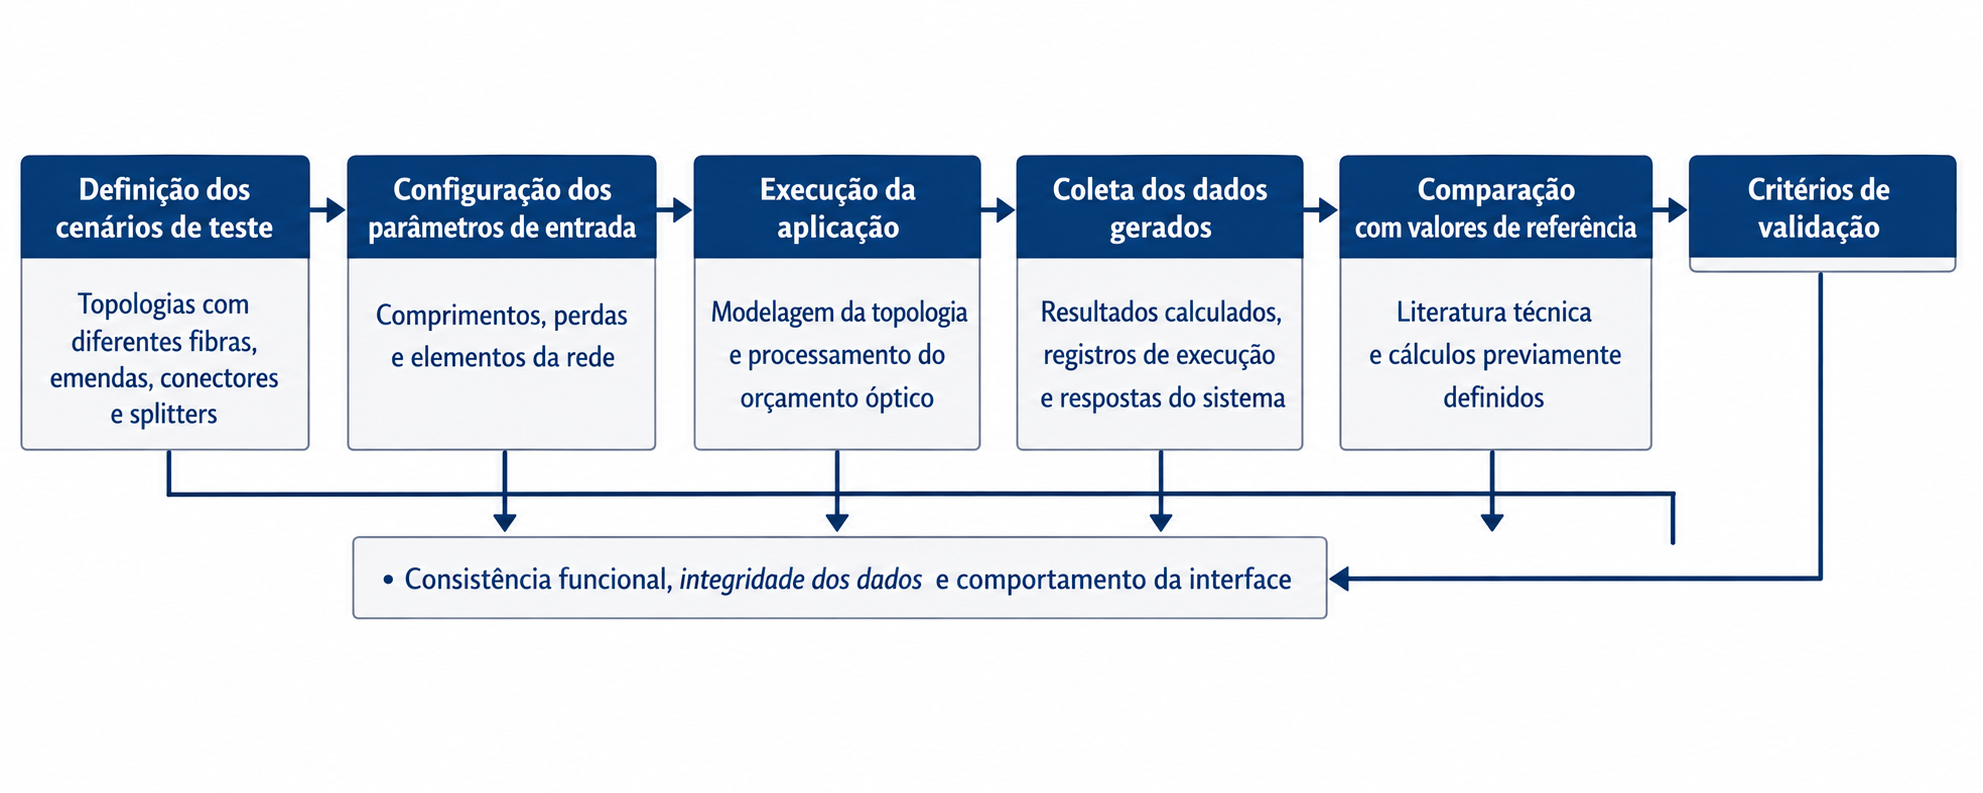
\includegraphics[width=\textwidth]{images/fluxo_validacao.png}
		\par\footnotesize Fonte: Elaboração própria com auxilio de IA.
    }
\end{figure}

A avaliação da solução considerará a correção das operações de modelagem, a consistência dos valores de orçamento óptico, o comportamento frente a diferentes estruturas de rede e a integridade dos dados. A ferramenta será considerada adequada quando os cenários apresentarem diferenças dentro da tolerância definida, os status calculados forem coerentes com as margens de referência e os projetos puderem ser persistidos e recuperados sem perda dos parâmetros relevantes.

\subsection{Avaliação de desempenho e escalabilidade visual}

O desempenho será analisado por meio de topologias com tamanhos crescentes, registrando a quantidade de nós, enlaces e caminhos \gls{olt}-\gls{onu}. Para cada tamanho serão coletadas várias execuções do endpoint de cálculo, considerando a média, o pior caso e os percentis de tempo. Quando possível, o tempo do \textit{backend} será separado do tempo de atualização visual no navegador. Essa avaliação permitirá identificar o comportamento do protótipo em redes maiores sem transformar uma medição pontual em garantia de desempenho para redes extremamente densas.

A interface utiliza D3.js com elementos \gls{svg}, escolha adequada para a manipulação customizada de nós, enlaces, zoom e arraste, mas que pode apresentar limitações à medida que a quantidade de elementos aumenta. Caso os testes indiquem degradação relevante, a renderização incremental, a agregação visual ou a adoção de Canvas/WebGL constituem alternativas para trabalhos futuros.

\subsection{Limitações e ameaças à validade}

O cálculo manual utiliza os mesmos pressupostos físicos e parâmetros de perda definidos no modelo, podendo reproduzir uma hipótese incorreta sem detectar limitações dos valores adotados. Além disso, os experimentos não substituem medições de campo, e a análise de desempenho depende do ambiente de execução. A utilização de arquivos \gls{json} simplifica a interoperabilidade e a persistência local, mas não avalia colaboração simultânea ou controle de conflitos em escala. Por fim, as classes ópticas B+, C+ e C++ são discutidas na fundamentação, enquanto a versão avaliada permite informar diretamente os parâmetros de potência e sensibilidade dos equipamentos, sem seleção automática por classe.

Do ponto de vista ético, o trabalho limita-se à análise técnica de um sistema computacional, sem envolvimento de dados pessoais ou participantes humanos, adotando princípios de integridade científica, rastreabilidade dos testes e transparência na apresentação dos resultados.
